%%%%%%%%%%%%%%%%%%%%%%%%%%%%%%%%%%%%%%%%%%%%%%%%%%%%%%%%%%%%%%%%%%%%%%%%%%%%%%%%%%%%%%%%%%%%%%
\section{回路設計}
設計した回路について選定の理由や仕様について以下に示す.
また使用する部品の一覧を表\ref{tab:c_parts}に示す.

\subsection{マイコンの選定}
設計した回路を図\ref{c_raspberry},図\ref{c_arduino}に示す.
マイコンとして「Raspberry Pi3 Model B(以下 RPi)」と「Arduino uno R3(以下 Arduino)」を使用する.それぞれが,統合・画像処理・モータ制御,
センサ処理,を行う.RPiでは複雑な処理を行う上で,LinuxOSの支援を受けることができ有利である.さらに,処理速度がCPU 1.2[GHz],
メモリ1[GB]とArduinoの16[MHz]・32[KB]と比べても大きく優れている.これは,並列処理や高速な画像処理に適している.このような理由からRPi
を採用した.

また ,RPiはアナログI/Oポートを持っておらず,アナログ電圧出力を行うセンサ類の処理が困難である.そこで,アナログ・ディジタルI/Oポートを
持つArduinoにセンサ類の処理を担わせることとした.ただし,要求されるアナログI/Oポート数が後述の$I^2 C$通信を使用しても足りない.そこで
Arduino用16チャンネル・アナログ・マルチプレクサを使用することで増設を行った.
\begin{table}[h]
  \centering
  \caption{回路用部品表}
  \begin{tabular}{|l|l|r||l|} \hline
    タイプ & 部品名 & 数 & 用途 \\ \hline \hline
     マイコン & Raspberry Pi3 & 1& 統括・画像処理・モータ制御 \\ \cline{2-4}
     & Arduino uno R3& 1 & センサ類の処理 \\ \hline
     DCモータ & AO-8014 & 2 & 駆動用 \\ \cline{2-4}
      & TAMIYA ミニモータ & 1&アーム用  \\ \hline
    モータドライバ& MD10C-R3 & 2& タイヤ用 \\ \cline{2-4}
      &  TA7291P&1 &アーム用 \\ \hline
   アナログマルチプレクサ & CD74HC4067 & 1 & ArduinoアナログI/Oピン増設 \\ \hline
    $I^2 C$通信用変換モジュール&PCA9306&1&$I^2 C$通信\\ \hline
     赤外線測距センサ& GP2Y0A02YK &6&中距離センサ\\ \hline
      ToF近距離センサ& VL6180x&3&近接センサ \\ \hline
     カメラモジュール&P5V04A&1&画像処理\\ \hline
     3軸加速度センサ&KXR94-2050&1&自己位置推定\\ \hline
     3軸ジャイロセンサ&BGD20&1&自己位置推定\\ \hline
    DCDCコンバータ&LT8697&1& 7.2[V]→5.0[V]2500[mA]降圧レギュレータ\\ \cline{2-4}
       &BTD05-05S200D&1&7.2[V]→5.0[V]2000[mA]降圧レギュレータ\\ \hline
    コンデンサ&電解コンデンサ 47[$\mu$F]&2&電源安定化\\ \cline{2-4}
            &セラミックコンデンサ 0.1 $\mu$ ]&9&センサ信号安定化\\ \hline
   バッテリー&POWER MAX 4000 Ni-MH&1&電源バッテリー 7.2[V]4200[mAh]\\ \hline
                 
  \end{tabular}
  \label{tab:c_parts}
\end{table}
\newpage
\begin{figure}[h]
 \centering
 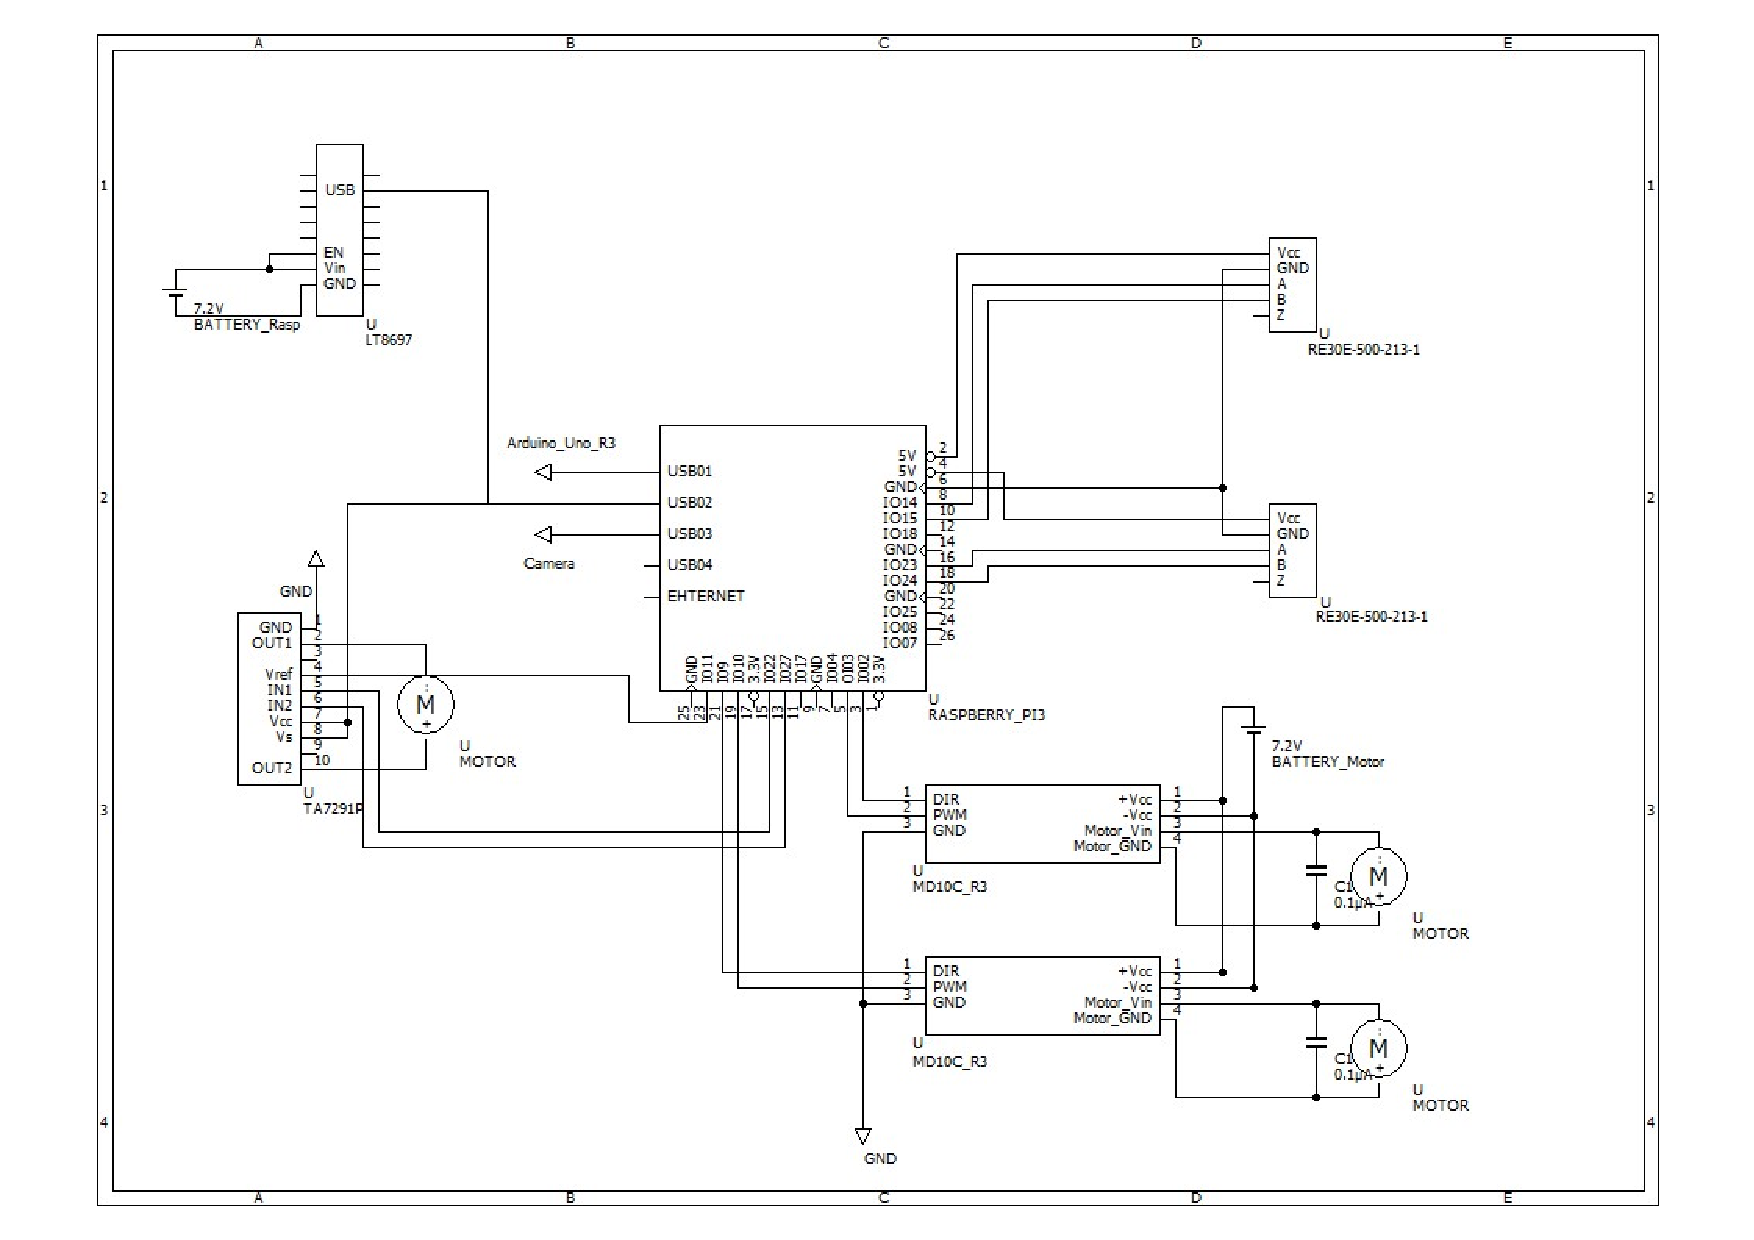
\includegraphics[clip,scale=0.35]{./picture/RCR_raspberryPi3.pdf}
    \caption{Raspberry Pi3 接続回路図}
    \label{c_raspberry}
\end{figure}

\begin{figure}[h]
 \centering
 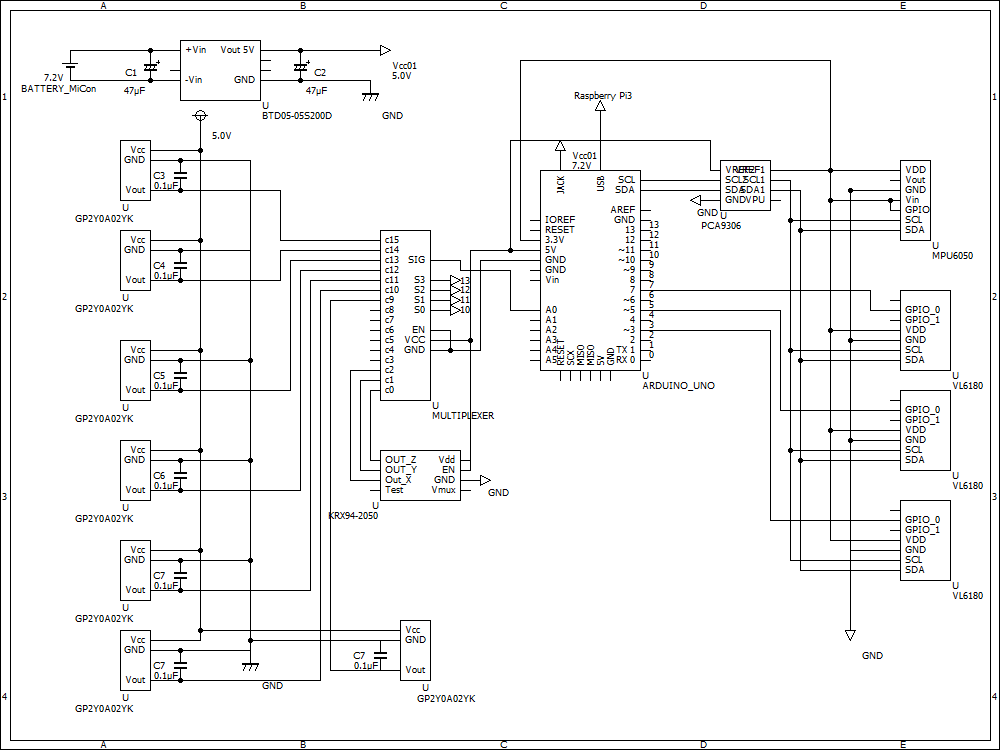
\includegraphics[clip,scale=0.35]{./picture/RCR_arduino_02.png}
    \caption{Arduino unoR3 接続回路図}
    \label{c_arduino}
\end{figure}
\newpage

%%%%%%%%%%%%%%%%%%%%%%%%%%%%%%%%%%%%%%%%%%%%%%%%%%%%%%%%%%%%%%%%%%%%%%%%%%%%%%%%%%%%%%%%%%%
\newpage
\subsection{モータドライバ}
モータドライバは「MD10C R3」(図\ref{MD10C})を両輪駆動用として2つ使用し,
「TA7291P」(図\ref{TA7291P})をアーム用として使用する.
各仕様を下に示す.

[MD10C R3](駆動用)
\begin{itemize}
 \item モータ電源電圧 : DC 5[V]$〜$25[V]
 \item モータ最大電流 : 13[A]
 \item ロジック用電源 : モータ用より供給
 \item ロジック電圧   : DC 5[V] or 3.3[V]
\end{itemize}

[TA7291P](アーム用)
\begin{itemize}
 \item モータ電源電圧 : DC 0[V]$〜$20[V]
 \item モータ最大電流 : 1.0[A]
 \item ロジック電圧 : DC 4.5[V]$〜$20[V]
\end{itemize}
\begin{figure}[h]
 \centering
 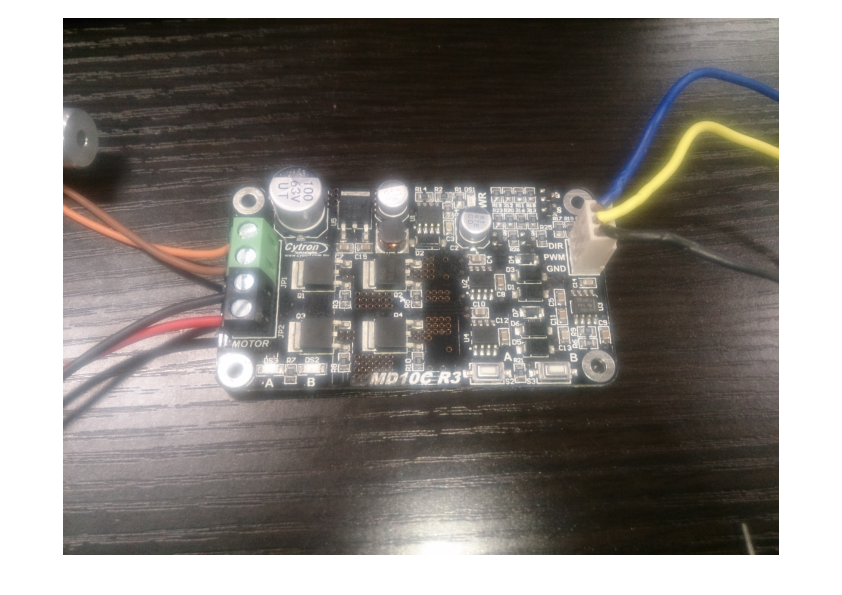
\includegraphics[width=0.5\hsize]{./picture/MD10C.png}
    \caption{MD10C R3}
    \label{MD10C}
\end{figure}
\begin{figure}[h]
 \centering
 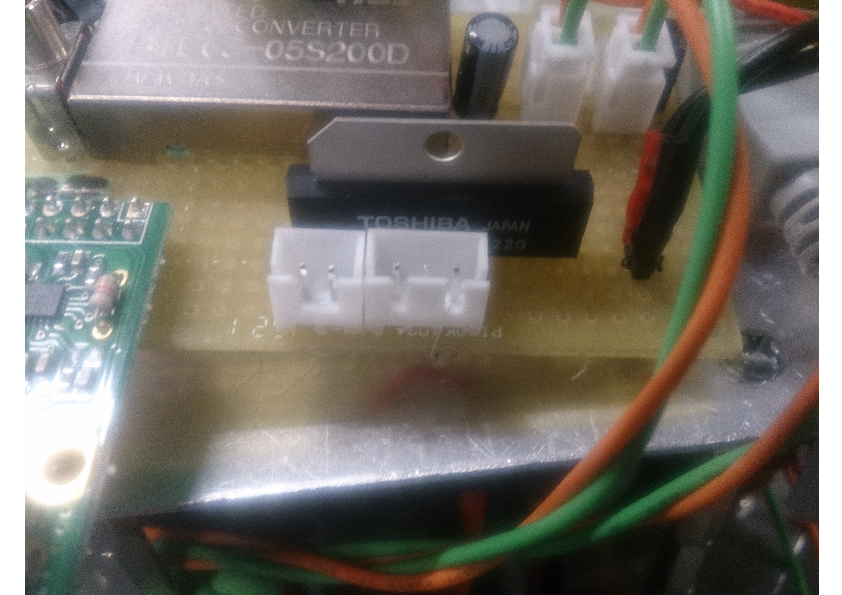
\includegraphics[width=0.5\hsize]{./picture/TO.png}
    \caption{TA7291P}
    \label{TA7291P}
\end{figure}

%%%%%%%%%%%%%%%%%%%%%%%%%%%%%%%%%%%%%%%%%%%%%%%%%%%%%%%%%%%%%%%%%%%%%%%%%%%%%%%%%%%%%%%%%%%%%%
\newpage
\subsection{センサ仕様}
ロボットに搭載されているセンサは以下である.
\begin{itemize}
 \item 赤外線測距センサ : GP2Y0A025YK : 有効距離$20 〜 150$[cm]
 \item ToF近距離センサ : VL6180x    : 有効距離$5 〜 20$[cm]
 \item 3軸加速度センサ : KXR94-2050 : [ x, y, z ]軸 加速度出力
 \item ジャイロセンサ : BGD20 : [ x, y, z ]軸 角加速度出力
 \item カメラモジュール : P5V04A : RPi用カメラ
\end{itemize}
%%%%%%%%%%%%%%%%%%%%%%%%%%%%%%%%%%%%%%%%%%%%%%%%%%%%%%%%%%%%%%%%%%%%%%%%%%%%%%%%%%%%%%%%
\subsubsection{測距センサ}  
測距センサは本体周囲にPSDセンサを7つ,前方にToF近接センサを3つ搭載する.(図\ref{Distance})これは自律行動の際に,
周辺環境,特に各種ポールを把握するために用いる.このとき,近接センサは$I^2 C$通信によって使用する.
センサの仕様については実験を行ったので\ref{psdex}に示す.

また,各測距センサには信号のノイズを吸収し安定化させるために$0.1[\mu $F]のセラミックコンデンサを接続する.
これは,コンデンサの持つ交流成分のみを吸収し,直流成分を通すというローパスフィルタ的特徴を利用したものである.

\begin{figure}[b]
 \centering
 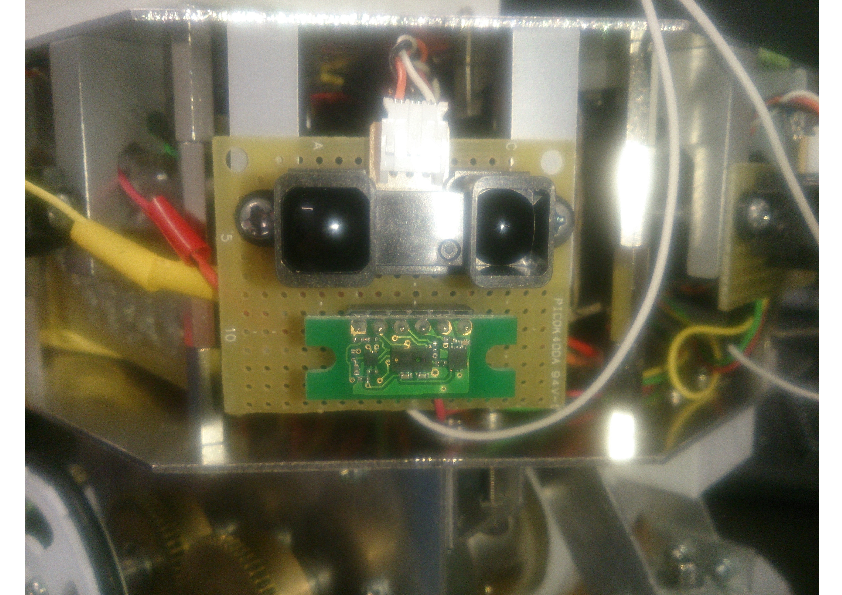
\includegraphics[width=0.5\hsize]{./picture/Distance.png}
    \caption{上:PSDセンサ 下:ToFセンサ}
    \label{Distance}
\end{figure}
%%%%%%%%%%%%%%%%%%%%%%%%%%%%%%%%%%%%%%%%%%%%%%%%%%%%%%%%%%%%%%%%%%%%%%%%%%%%%%%%%%%%%%%%%%%%
\subsubsection{3軸加速度・ジャイロセンサモジュール}
加速度センサは[ x, y, z ]軸におけるロボットの加速度を測定するものである.

ジャイロセンサは[ x, y, z ]軸まわりの角加速度を測定するものである.(図\ref{jairo})

我々はこれらをロボットの自己位置推定に用いる.特にジャイロセンサについては,
ロボット本体の直進走行制御に使用する.詳細は\ref{algo}において説明する.
\begin{figure}[t]
 \centering
 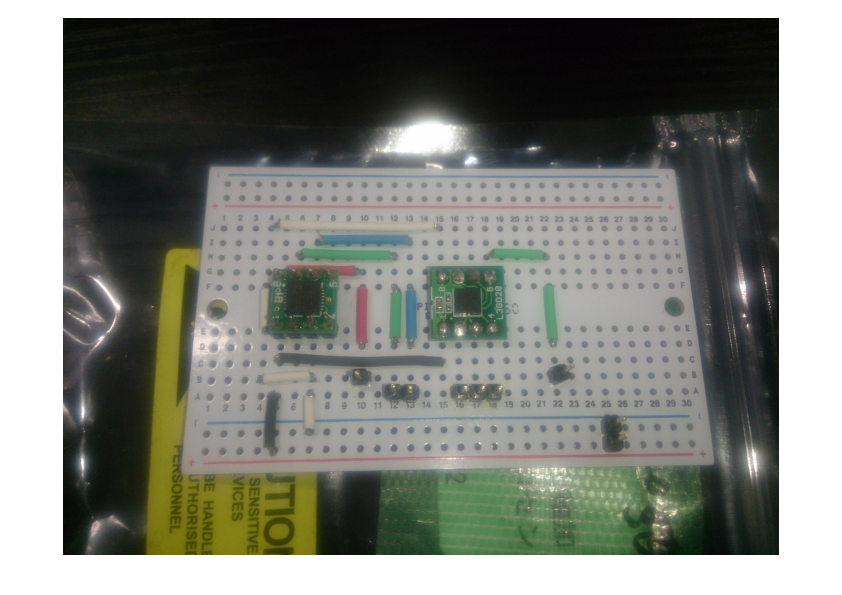
\includegraphics[width=0.4\hsize]{./picture/jairo.png}
    \caption{3軸加速度・ジャイロセンサモジュール}
    \label{jairo}
\end{figure}
\subsection{電源回路}
電源回路は各回路図の左上に示している.\\
バッテリーはひとつしか搭載しないが,RPiとArduinoでは定格電流値が異なるために同一の電源は使用できない.
そこで,それぞれに降圧レギュレータとしてDCDCコンバータを用いてバッテリーからの供給電源を
分電することとした.各仕様を下に示す.
また,実際に作成した電源回路を図\ref{dengen}に示す.

[LR8697](RPi・モータ用)
\begin{itemize}
 \item 電源電圧 : DC 6.0[V]$〜$42.0[V]]
 \item 出力電圧 : DC 5.0[V]]
 \item 出力電流 : 2.5[A]
\end{itemize}

[BTD05-05S200D](Arduino・センサ用)
\begin{itemize}
 \item 電源電圧 : 4.5-9.0[V]
 \item 出力電圧 : 5.0[V]
 \item 出力電流 : 2000[mA]
\end{itemize}
\begin{figure}[t]
 \centering
 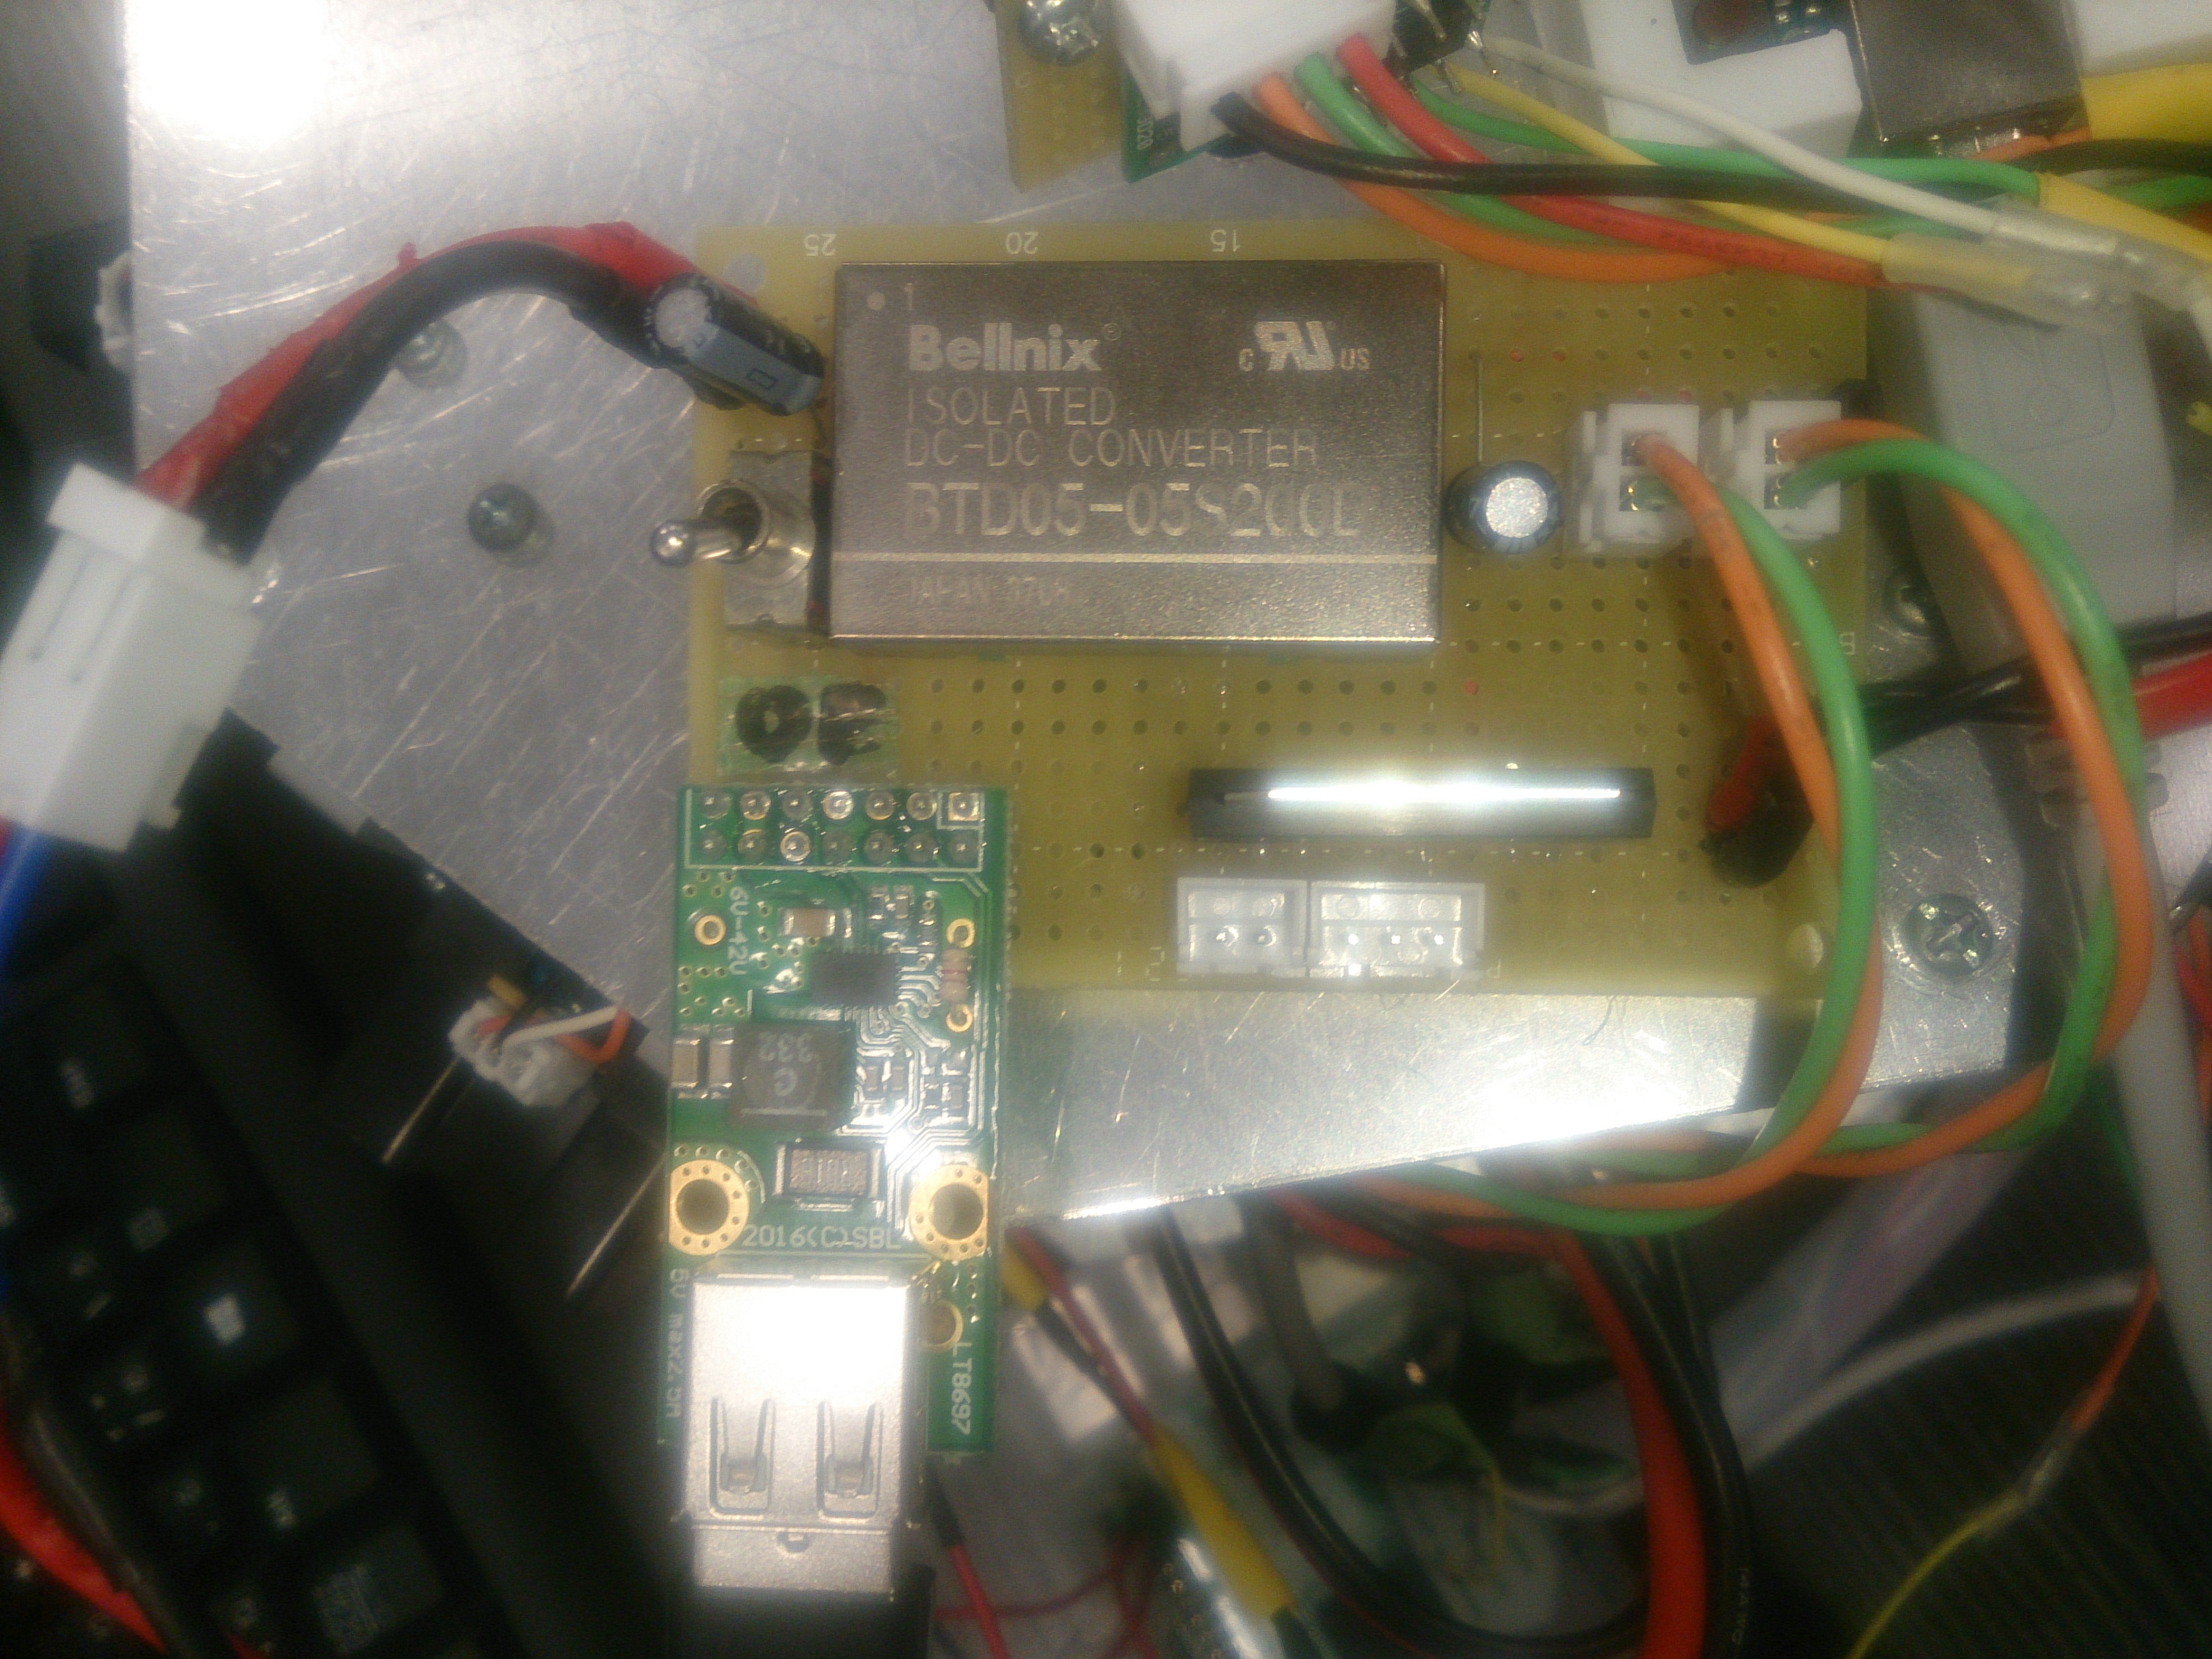
\includegraphics[width=0.4\hsize]{./picture/dengen.png}
    \caption{電源回路モジュール}
    \label{dengen}
\end{figure}
%%%%%%%%%%%%%%%%%%%%%%%%%%%%%%%%%%%%%%%%%%%%%%%%%%%%%%%%%%%%%%%%%%%%%%%%%%%%%%%%%%%%%%%%%%%
\newpage
\subsection{$I^2 C$通信}
今回,我々のロボットには測距センサを始めとする複数のセンサが搭載されている.これらの殆どがアナログ出力
であるが,ArduinoのアナログI/Oポートは6つしかなく,要求を満たしていない.

そこで,$I^2 C$通信を用いることとする.これは,$I^2 C$通信がパーティライン構成が可能となっており
,1つのマスタで複数のスレーブデバイスと通信することが可能であるからである.概要を以下に示す.
\begin{enumerate}
 \item マスタ側(Arduino)とスレーブ側(n個のセンサ等)を明確に分け,各スレーブに異なるアドレスを割り振る.
 \item マスタ側が、Start Conditionを出力し続いてアドレスとRead/Write要求を出力する.
 \item 全スレーブがこの時のSCLのクロックを元にSDAのデータを受信し、SSPADDレジスタにセットされたアドレスと一致したデバイスだけが、その後の送受信を継続する.
 \item 受信した側がデータを受信完了すると自動的にACKビットを返送し、同時にSSP割込みを発生する.
 \item これをマスタがStop Conditionを出力するまで続ける.
\end{enumerate}

本ロボットでは,近接センサ・ジャイロセンサについて$I^2 C$通信を行うこととする.また,Arduinoと各デバイスは
ArduinoのSDA・SCLポートを使用することで通信が可能となる.これを実現するためにArduino用$I^2 C$バス用双方向電圧レベル変換モジュール
(図\ref{level})を使用して接続した.接続の方法は回路図に示している.

\begin{figure}[b]
 \centering
 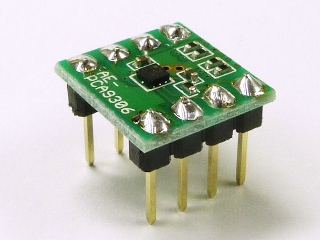
\includegraphics[width=0.4\hsize]{./picture/level.png}
    \caption{レベル変換モジュール}
    \label{level}
\end{figure}
%%%%%%%%%%%%%%%%%%%%%%%%%%%%%%%%%%%%%%%%%%%%%%%%%%%%%%%%%%%%%%%%%%%%%%%%%%%%%%%%%%%%%%%%%%%%%%
